%% LyX 2.3.6 created this file.  For more info, see http://www.lyx.org/.
%% Do not edit unless you really know what you are doing.
\documentclass[english]{article}
\usepackage[T1]{fontenc}
\usepackage[latin9]{inputenc}
\usepackage{babel}
\usepackage{graphicx}
\usepackage[unicode=true]
 {hyperref}

\makeatletter

%%%%%%%%%%%%%%%%%%%%%%%%%%%%%% LyX specific LaTeX commands.
%% Because html converters don't know tabularnewline
\providecommand{\tabularnewline}{\\}

\makeatother

\begin{document}
\title{Audio Fading, Mixing and Amplification}

\maketitle
\begin{figure}
\caption{Audio Mixing and Amplification}

\centering{}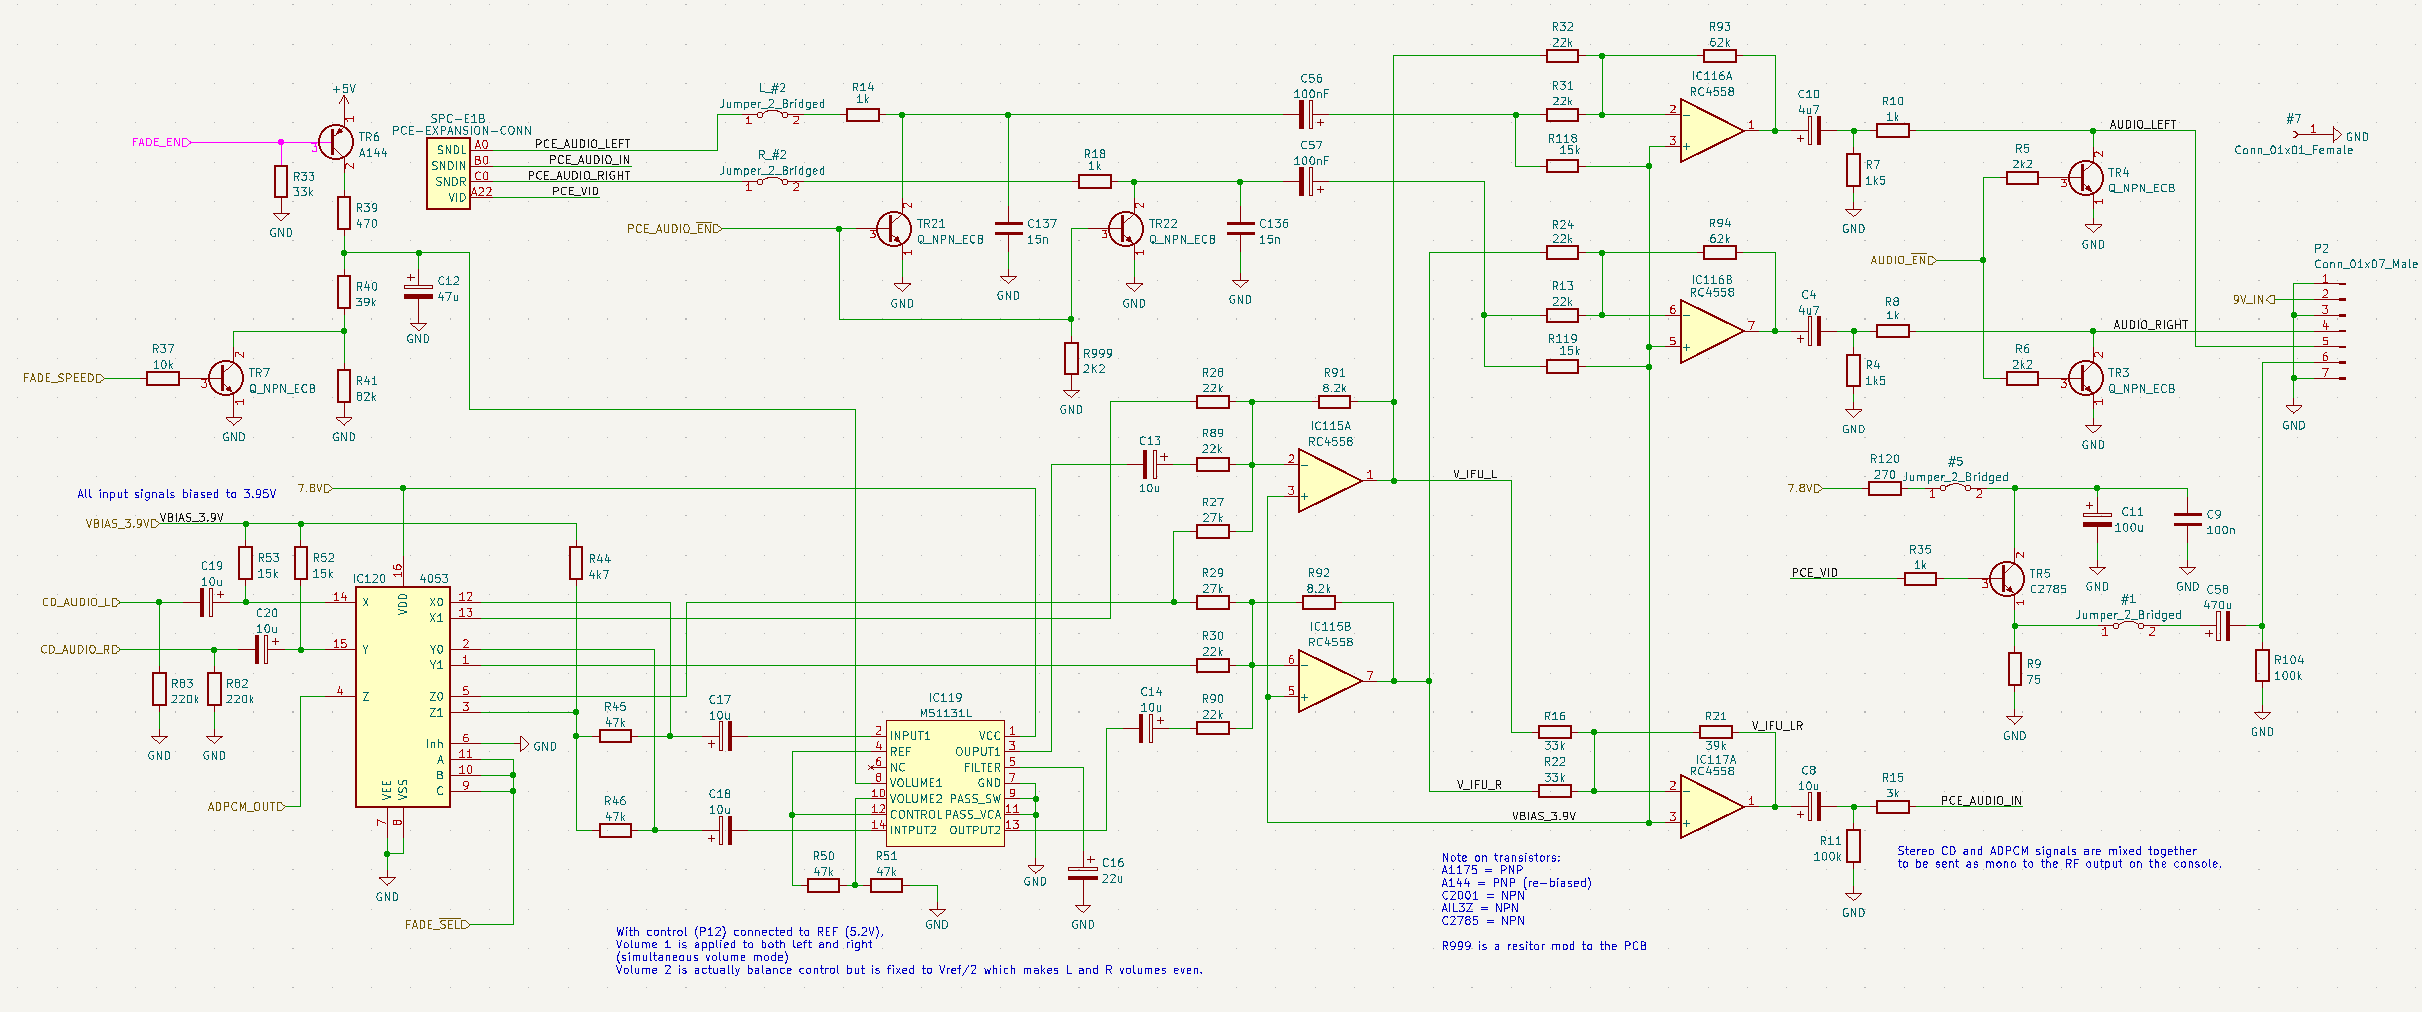
\includegraphics{AudioMixingAndAmplification}
\end{figure}


\section{Audio Fading Circuit}

The ADPCM signal and the CD audio left and right channels can be faded
out at 2 different rates via register 180Fh; 2.5s or 6s. In normal
operation i.e. when not fading is applied, TR6 (A144) is constantly
saturated by pulling the base to GND via R33 and this allows C12 to
charge to 5V via R39.\linebreak{}
\linebreak{}
When fading is enabled, the IC output (which I expect to be an open
collector output) to pull up the base to 5V and thus stop sauration.
This will have the effect of discharging C12 through R40 in fast fading
mode and through R40 and R41 in slow fading mode. The fading mode
is controlling TR7: when the IC pulls the base up, it is saturated
which makes it short R41 giving the fast fading mode. When the IC
output is floating, the base no longer receives current and the transistor
is open giving the slow fading mode.

\begin{figure}

\caption{C12 Charging and Discharging}

\centering{}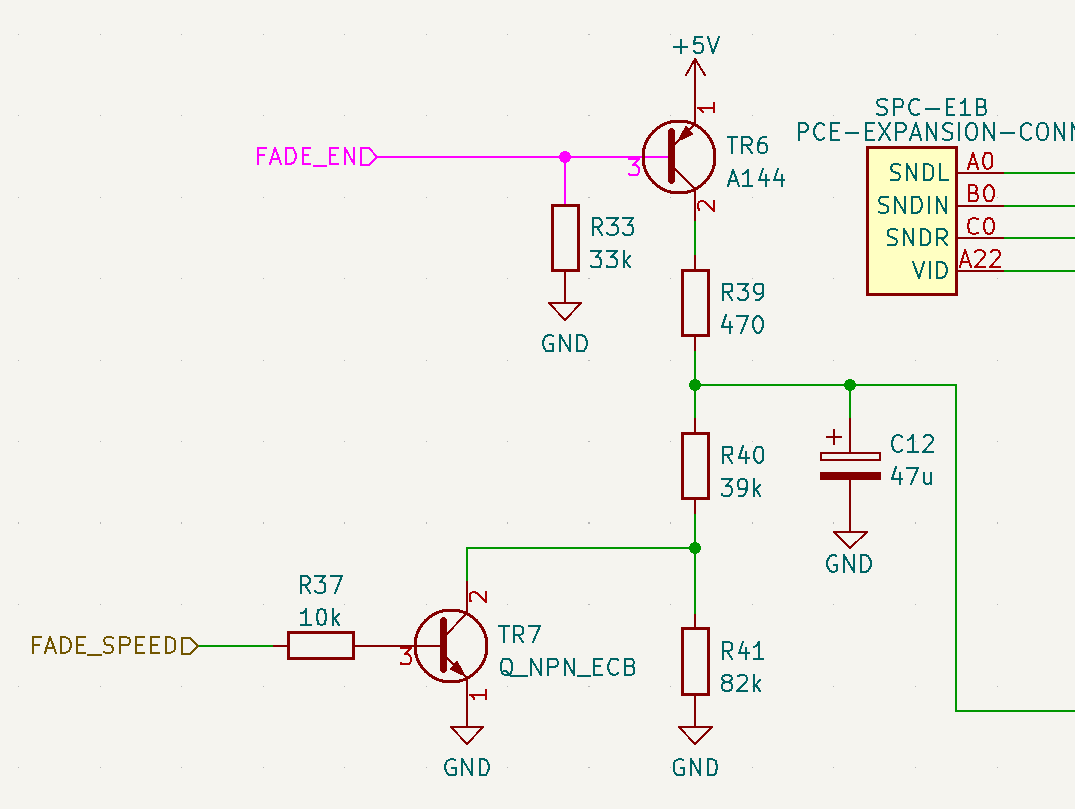
\includegraphics{C12_ChargingDischarging}
\end{figure}


\subsection{C12 Charging}

The time constant for the charging of C12 is:

\[
\tau=R39\times C12=470\times47\times10^{-6}=22.09ms
\]
It means that we can consider C12 fully charged after approximately
$3\tau$ or 66ms. Therefore, the sound will recover pretty quickly
as soon as fading is disabled.

\subsection{C12 Discharging}

Discharging will happen at 2 different rates based on the state of
TR7. TR7 close = fast discharge through R40; TR7 opened = slow discharge
through R40 and R41.\linebreak{}
\linebreak{}
The time constant for the fast discharging of C12 is:

\[
\tau_{1}=R40\times C12=39\times10^{3}\times47\times10^{-6}=1833ms
\]
It means that we can consider C12 fully discharged after approximately
$3\tau$ or 5499ms.\linebreak{}
\linebreak{}
The time constant for the slow discharging of C12 is:

\[
\tau_{2}=(R40+R41)\times C12=(39+82)\times10^{3}\times47\times10^{-6}=5687ms
\]
It means that we can consider C12 fully discharged after approximately
$3\tau$ or 17061ms.\linebreak{}
\linebreak{}
We can see that these values are a lot greater than what is mentioned
in the CD-ROM BIOS documentation which mentions 2.5s and 6s. This
is what what we will explain in the section covering the volume chip,
M51131L.\linebreak{}
\begin{figure}
\caption{Fast and Slow Discharge Graphs}

\begin{centering}
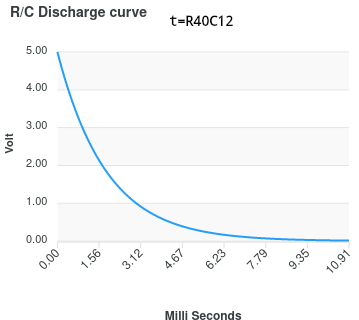
\includegraphics{R40C12}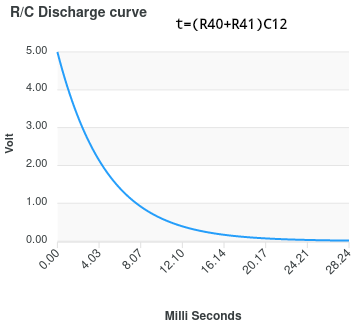
\includegraphics{R40R41C12}
\par\end{centering}
\href{https://www.redcrab-software.com/en/Calculator/Electrics/C-Discharge-State}{Graphs generated here!}
\end{figure}


\subsection{BU4053 - Analogue Switch}

\begin{figure}

\caption{Analogue Switch}

\centering{}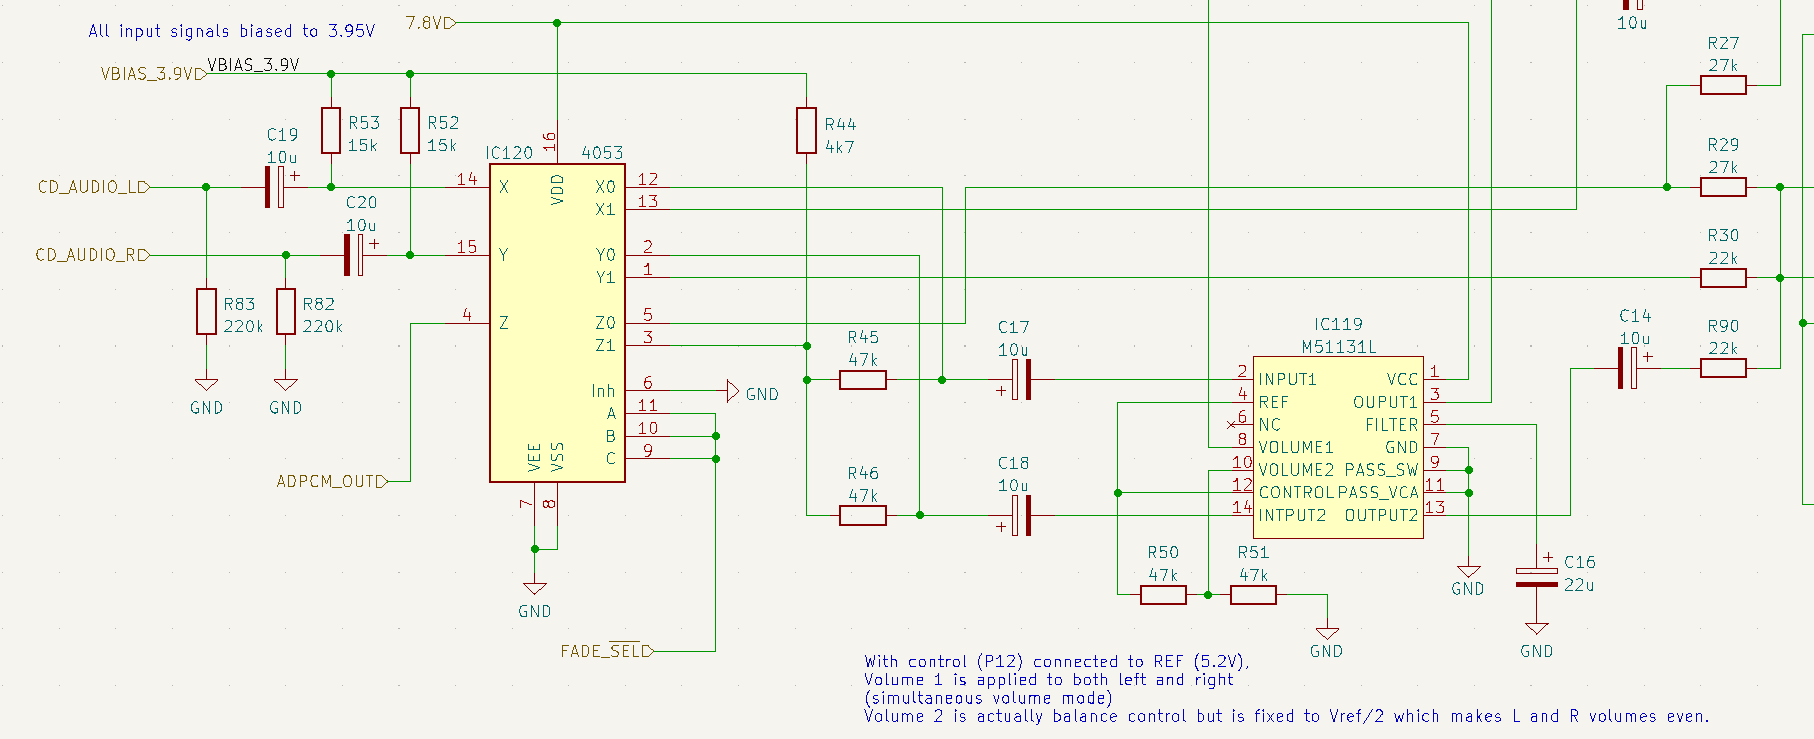
\includegraphics{AnalogueSwitch}
\end{figure}
IC4053 is a 3 channel 2:1 analogue switch. Pin X, Y and Z are the
inputs pins for the stereo signals from the CD-ROM and the ADPCM signal.
ADPCM already has 3.9V biasing applied, however the CD-ROM signals
are coupled with C19 and C20 to remove any biasing that may be present
from the CD-ROM but then get biased to 3.9V via R53 and R52. When
FADE\_SELn connected to pin A, B and C is high, the signals are passed
to the rest of the circuitry as is. When FADE\_SELn is low, the signals
are fed to the volume control IC instead, MM51131L. Note that Inh
is tied to GND to always enable it. 

\subsection{Register 180Fh}

This is the register that controls the fading. From looking at the
bios, there is only 1 place where this register is written to with
value 0Fh. From looking at IC connections and using exisitng observations
from Charles MacDonald, the following conclusion can be made: Main
IC P81 is FADE\_SELn and is connected to bit1, Main IC P80 is FADE\_SPEED
and is connected to bit2, Main IC P79 is FADE\_EN and is connected
to bit3. 
\begin{table}
\caption{Register 180Fh}

\centering{}%
\begin{tabular}{|c|c|c|c|}
\hline 
bit3:FADE\_EN & bit2:FADE\_SPEED & bit1:FADE\_SELn & Audio State\tabularnewline
\hline 
\hline 
0 & x & x & No fading\tabularnewline
\hline 
1 & 0 & 0 & 8 second fading\tabularnewline
\hline 
1 & 0 & 1 & No fading (but C12 is discharging slowly)\tabularnewline
\hline 
1 & 1 & 0 & 2.5 second fading\tabularnewline
\hline 
1 & 1 & 1 & No fading (but C12 is discharging fast)\tabularnewline
\hline 
\end{tabular}
\end{table}


\subsection{M51131L - Volume Control IC}

\begin{figure}

\caption{M51131L Attenuation against Volume Control Voltage}

\centering{}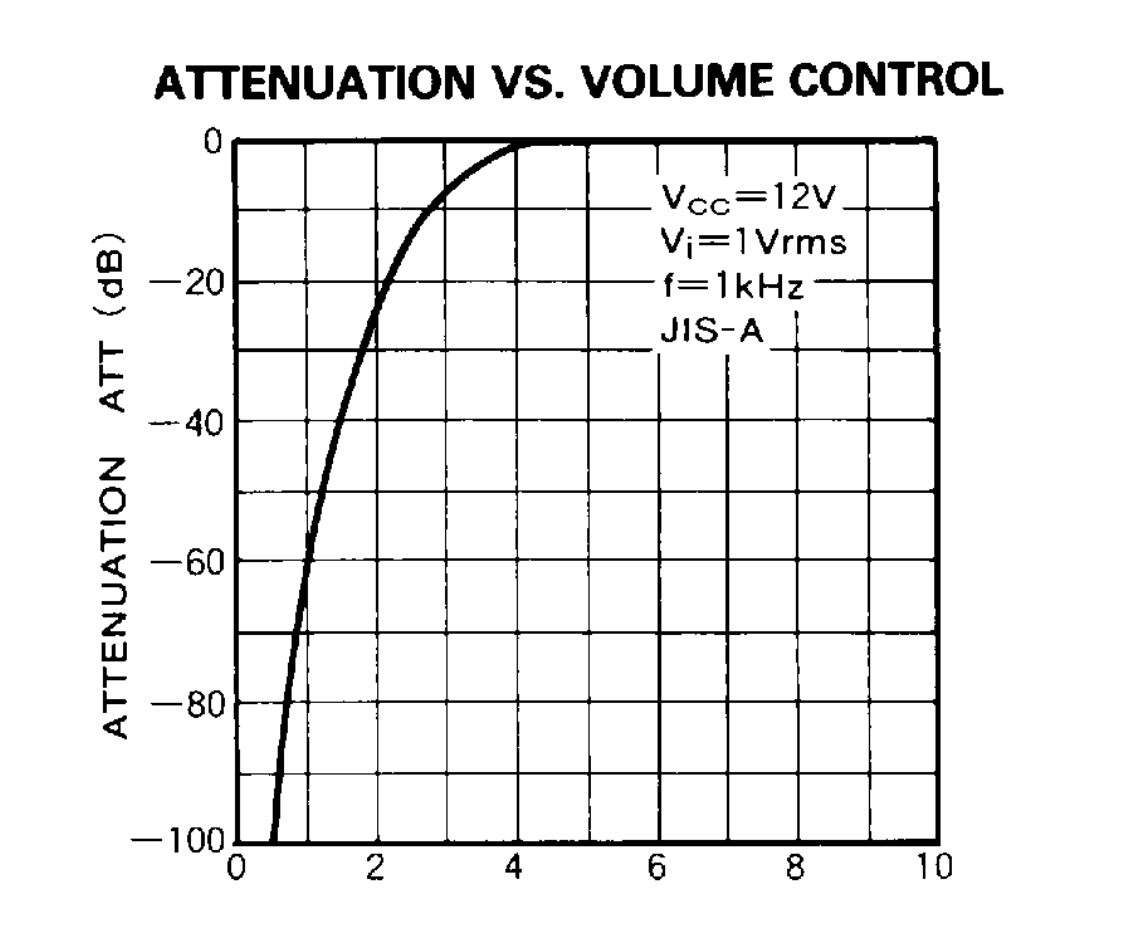
\includegraphics{M51131L_Attenuation}
\end{figure}
With control pin (P12) connected to REF (5.2V), Volume 1 is applied
to both left and right channels called simultaneous volume mode in
datasheet and Volume 2 is actually used for balance control. In this
case, Volume 2 is set to Vref/2 which makes L and R volumes equal.
Attenuation is maximum when C12 voltage reaches 0.5V. Based on C12
discharge rates the maximum attenuation will be reached in 4.22s with
$\tau_{1}$ and 13.08s with $\tau_{2}$. The CD-BISO documentation
mentions 2.5 and 6 seconds but Charles McDonald mentions 2.5s and
8s which are more in-line with the calculations. We can see that if
we use the latter values, voltage at C12 reaches 1V with 60dB attenuation
from 4.2V (no attenuation) after 2.5s with $\tau_{1}$ and 8s with
$\tau_{2}$ which implies that the BIOS documentation is inaccurate.

\section{ADPCM and CD Audio Amplification}

\subsection{IC115A\&B - Adders}

The ADPCM signal and the CD audio channels are fed to dual op-amp
IC115 configured as an adder with negative gain. From looking at the
resistor values, we can see that that gain will be less than 1 and
that ADPCM signal will be amplified a bit less than the CD audio channels.
\begin{figure}
\caption{IC115A\&B ADPCM and CD Audio Mixing}

\centering{}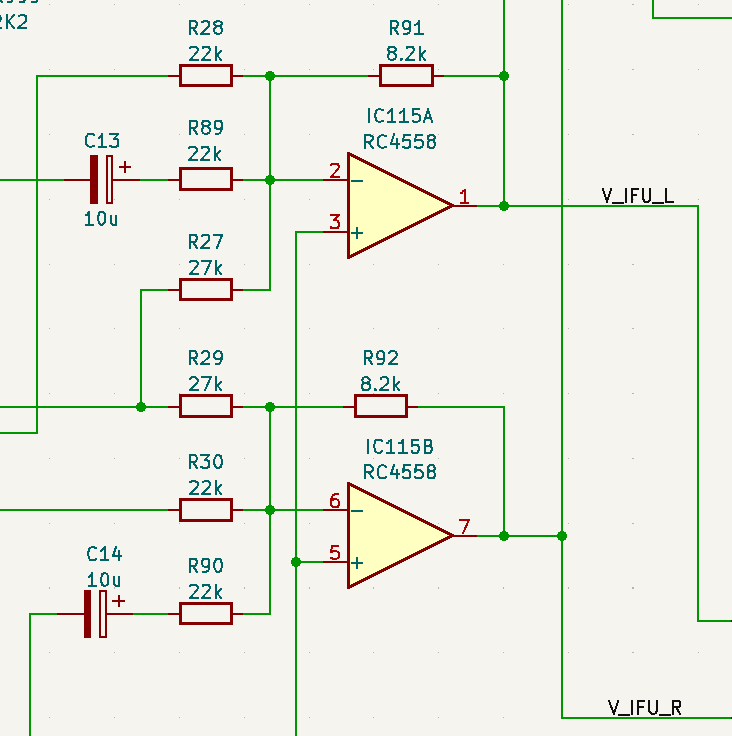
\includegraphics{IC115A&B}
\end{figure}
At DC level, we will omit the audio signals and only include the biasing
voltages. 

\[
\frac{V_{BIAS}/(R52+R30)+V_{BIAS}/R29+V_{IFU_{R}}/R92}{1/(R52+R30)+1/R29+1/R92}=V_{BIAS}
\]

\[
\frac{3.9/(15k+22k)+3.9/27k+V_{IFU_{R}}/8.2k}{1/(15k+22k)+1/27k+1/8.2k}=3.9
\]

\[
3.9/37k+3.9/27k+V_{IFU_{R}}/8.2k=3.9/5.376k
\]

\[
V_{IFU_{R}}=3.9\times(1/5.376k-1/37k-1/27k)\times8.2k
\]

\[
V_{IFU_{R}}=3.9V
\]

\[
V_{IFU_{L}}=3.9V
\]
This confirms that biasing will be present on the output.\linebreak{}
\linebreak{}
At AC level, we will ignore the biasing voltages to concentrate on
the audio signals.

\[
\frac{V_{CD_{R}}/R30+V_{ADPCM}/R29+V_{FADE_{R}}/R90+V_{IFU_{R}}/R92}{1/R30+1/R29+1/R90+1/R92}=0
\]

\[
V_{CD_{R}}/22k+V_{ADPCM}/27k+V_{FADE_{R}}/22k+V_{IFU_{R}}/8.2k=0
\]

\[
V_{IFU_{R}}=-8.2k\times(V_{CD_{R}}/22k+V_{ADPCM}/27k+V_{FADE_{R}}/22k)
\]
\[
V_{IFU_{R}}=-\left(V_{CD_{R}}\times8.2/22+V_{ADPCM}\times8.2/27+V_{FADE_{R}}\times8.2/22\right)
\]
\[
V_{IFU_{L}}=-\left(V_{CD_{L}}\times8.2/22+V_{ADPCM}\times8.2/27+V_{FADE_{L}}\times8.2/22\right)
\]
When not in fading mode, gain is 8.2/22 = 0.373 for CD audio channels
and 8.2/27 = 0.304 for ADPCM signal. When fading is enabled, CD audio
channels are conencted directly to the M51131L inputs howver ADPCM
goes through a 47k resitor. I would expext this is due to the 150kohm
resistance on the M51131L inputs and therefore adding the 47k resistor
in series maintains the 22/27 ratio applied in normal mode between
CD and ADPCM as 150/(47+150) is close to 22/27. 

\subsection{IC117A - Adder}

\begin{figure}

\caption{IC117A Configured as Adder}

\centering{}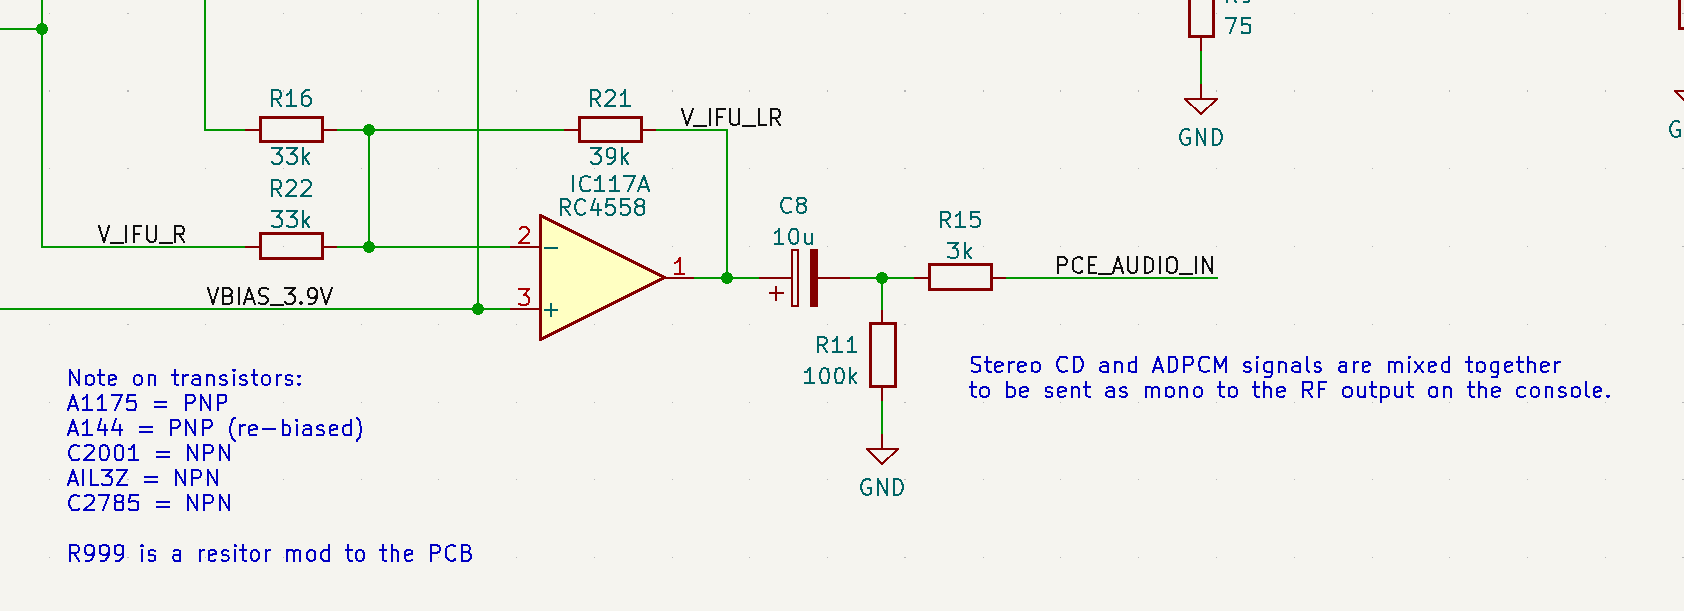
\includegraphics{IC117A}
\end{figure}
This opamp mixes the IFU signals (CD and ADPCM) to send then back
as mono to the PC-Engine to be present on the RF connector (which
is always mono).\linebreak{}
\linebreak{}
At DC level, we will omit the audio signals and only include the biasing
voltages.

\[
\frac{V_{IFUL}/R16+V_{IFUR}/R22+V_{IFULR}/R21}{1/R16+1/R22+1/R21}=V_{BIAS}
\]
\[
\frac{3.9/33k+3.9/33k+V_{IFULR}/39k}{1/33k+1/33k+1/39k}=3.9
\]
\[
V_{IFULR}=39k\times3.9\times(1/11.595k-1/33K-1/33K)
\]
\[
V_{IFULR}=3.9V
\]
At AC level, we will ignore the biasing voltages to concentrate on
the audio signals.

\[
\frac{V_{IFUL}/R16+V_{IFUR}/R22+V_{IFULR}/R21}{1/R16+1/R22+1/R21}=0
\]
\[
V_{IFUL}/33k+V_{IFUR}/33k+V_{IFULR}/39k=0
\]
\[
V_{IFULR}=-V_{IFUR}\times39/33-V_{IFUR}\times39/33
\]
Gain is 39/33 = 1.18 and signal is inverted which effectively cancels
out the inversion from the previous stage.

\subsection{PCE Audio Signals}

\begin{figure}

\caption{PCE Audio Signals}

\centering{}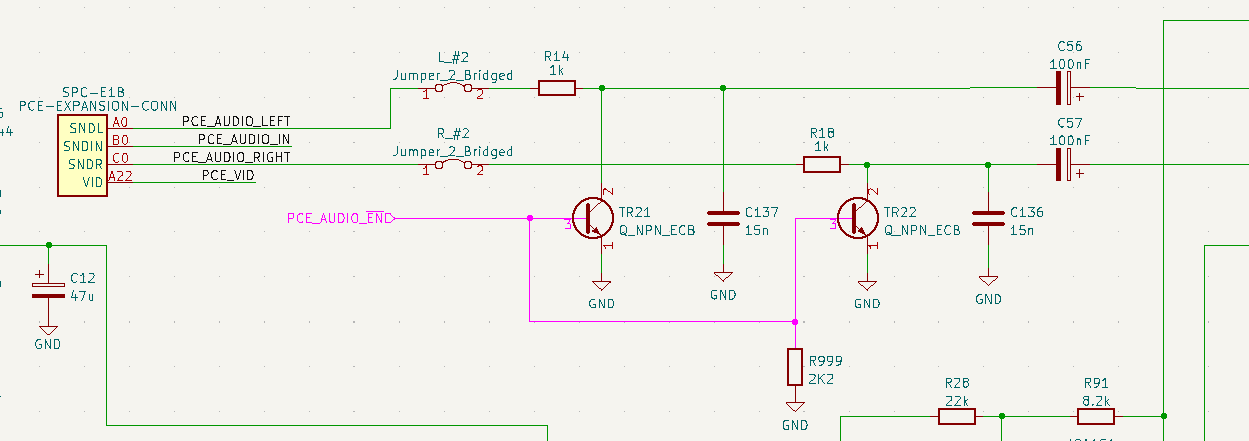
\includegraphics{PCE_Audio}
\end{figure}
PC-Engine console left and right audio signals are fed to the IFU
PCB in order to be mixed witht the CD and ADPCM signals. When the
console is not inserted or not powered, TR21 and TR22 are saturated
takin gthese signals to ground probably to stop picking up noise.
C56 and C57 are coupling capacitors removing any DC. Each channel
has a passive low-pass filter with $f_{C}=1/2\pi RC=1/\left(2\pi\times1k\times15\times10^{-9}\right)=10612Hz$.

\subsection{IC116A\&B - Adders}

\begin{figure}

\caption{IC116A\&B Adders}

\centering{}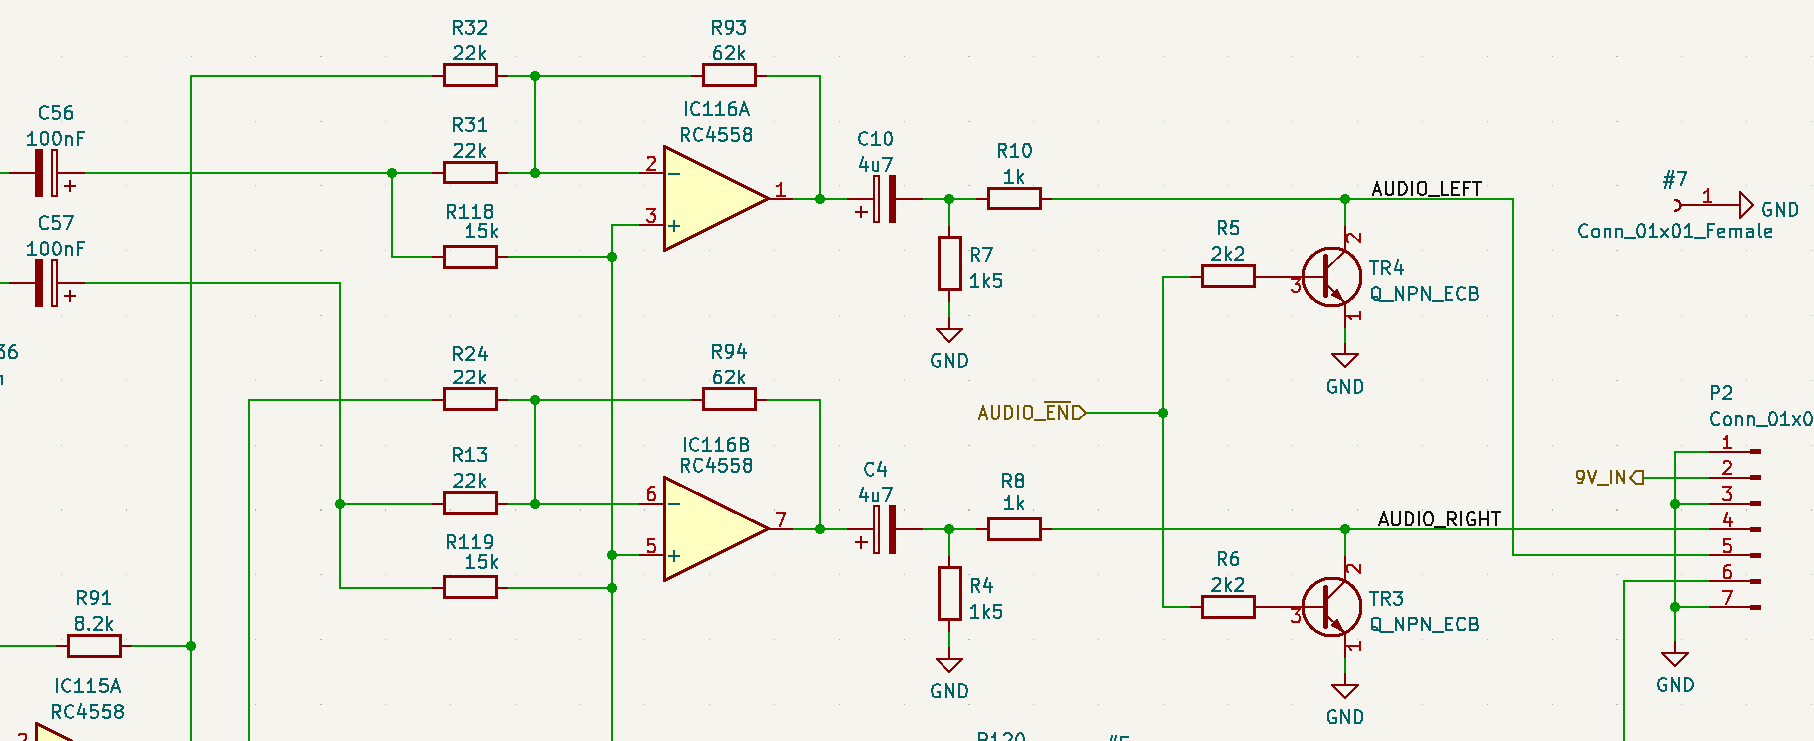
\includegraphics{IC116A&B}
\end{figure}
The purpose of these opamps are to mix the PCE audio signals with
the IFU audio signals. IC116A\&B are configured as an adder with negative
gain. From looking at the resistor values, we can see that that gain
will be greater than 1 in such way that it will restitute the CD audio
amplitude. ADCPM amplitude will be slightly less becaiuse of the previous
stage. \linebreak{}
\linebreak{}
At DC level, we will omit the audio signals and only include the biasing
voltages.

\[
\frac{V_{IFUL}/R32+V_{BIAS}/(R118+R31)+V_{AUDIOL}/R93}{1/R32+1/(R118+R31)+1/R93}=V_{BIAS}
\]
\[
3.9/22k+3.9/(15k+22k)+V_{AUDIOL}/62k=3.9\times(1/22k+1/(15k+22k)+1/62)
\]
\[
V_{AUDIOL}=62k\times3.9\times(1/11.285k-1/22K-1/37K)
\]
\[
V_{IFULR}=3.9V
\]
At AC level, we will ignore the biasing voltages to concentrate on
the audio signals.

\[
\frac{V_{IFUL}/R32+V_{PCEL}/R31+V_{AUDIOL}/R93}{1/R32+1/R31+1/R93}=0
\]
 
\[
V_{IFUL}/R32+V_{PCEL}/R31+V_{AUDIOL}/R93=0
\]
 
\[
V_{AUDIOL}=-R93\times(V_{IFUL}/R32+V_{PCEL}/R31)
\]
 
\[
V_{AUDIOL}=-V_{IFUL}\times62/22-V_{PCEL}\times62/22
\]
 Gain is 62/22 = 2.818. Multiplied by previous gain, we get $8.2/22\times62/22=1.05$
close enough to 1 (by 5\%). Before the signals leave the board, TR4
and TR3 can kill the signals when AUDIO\_ENn is high. This can come
from various sources like 5V not present, PC-Engine not plugged in
or main IC disabling audio. No documentation explain how the latter
could be achieved. 
\end{document}
